\documentclass{beamer}
\usepackage{pgfpages}
\usepackage[backend=bibtex]{biblatex}
\usepackage{multicol}
\setbeameroption{hide notes} % Only slides
%\setbeameroption{show only notes} % Only notes
%\setbeameroption{show notes on second screen=right} % Both
\bibliography{../../papers/references.bib}
\setbeamerfont{footnote}{size=\tiny}
%\AtEveryCitekey{\clearfield{title}}

%
% Choose how your presentation looks.
%
% For more themes, color themes and font themes, see:
% http://deic.uab.es/~iblanes/beamer_gallery/index_by_theme.html
%
\mode<presentation>
{
  \usetheme{Warsaw}      % or try Darmstadt, Madrid, Warsaw, ...
  \usecolortheme{default} % or try albatross, beaver, crane, ...
  \usefonttheme{default}  % or try serif, structurebold, ...
  \setbeamertemplate{navigation symbols}{}
  \setbeamertemplate{caption}[numbered]
} 

\usepackage[english]{babel}
%\usepackage[utf8x]{inputenc} %Doesn't play well with biblatex
\usepackage{amssymb}
\usepackage{bm}
\usepackage{color}
\usepackage{graphicx}

\newcommand{\red}[1]{{\color{red}{#1}}}
\newcommand{\ket}[1]{\left| #1 \right>}
\newcommand{\bra}[1]{\left< #1 \right|}
\newcommand{\braket}[2]{\left< #1 | #2 \right>}
\newcommand{\ketbra}[2]{\left| #1 \right> \left< #2 \right|}
\newcommand{\expect}[1]{\left< #1 \right>}
\newcommand{\fpij}{f_p(r_{ij})}
\newcommand{\vpij}{v_p(r_{ij})}
\newcommand{\Opij}{\mathcal{O}_{ij}^p}
\newcommand{\fOpij}{\sum\limits_{i<j}\sum\limits_p \fpij\Opij}
\newcommand{\fqkl}{f_q(r_{kl})}
\newcommand{\Oqkl}{\mathcal{O}_{kl}^q}
\newcommand{\fOqkl}{\sum\limits_{k<l}\sum\limits_q \fqkl\Oqkl}
\newcommand{\fOqklip}{\sum\limits_{k<l,\mathrm{ip}}\sum\limits_q \fqkl\Oqkl}
\newcommand{\fOqklquad}{\sum_{\substack{k<l\\ij \ne kl}}\sum\limits_q \fqkl\Oqkl}
\newcommand{\f}[2]{f_{#1}(r_{#2})}
\renewcommand{\O}[2]{\mathcal{O}_{#2}^{#1}}
\newcommand{\fO}[2]{\sum\limits_{#1} f_{#1}(r_{#2})\mathcal{O}_{#2}^{#1}}
\newcommand{\R}{\mathbf{R}}
\newcommand{\dt}{\Delta\tau}
\newcommand{\ti}{\bm{\tau}_i}
\newcommand{\tj}{\bm{\tau}_j}
\newcommand{\si}{\bm{\sigma}_i}
\newcommand{\sj}{\bm{\sigma}_j}

\title[Prospectus]{{\large Oral Comprehensive Exam/Prospectus:}\\Improved Trial Wave Function for Quantum Monte Carlo Calculations of Nuclear Systems}
\author[Cody L. Petrie]{Cody L. Petrie\\
Advisor: Kevin Schmidt}
\institute{Arizona State University}
%\date{}

\begin{document}

\begin{frame}
  \titlepage
\end{frame}

% Uncomment these lines for an automatically generated outline.
\begin{frame}{Outline}
  \tableofcontents
\end{frame}

% Commands to include a figure:
%\begin{figure}
%\includegraphics[width=\textwidth]{your-figure's-file-name}
%\caption{\label{fig:your-figure}Caption goes here.}
%\end{figure}

\section{Motivation}
\begin{frame}{Background}
\begin{itemize}
   \item $\left<H\right> = \left<\Psi\right|H\left|\Psi\right> = \int \Psi^*(\R) H \Psi(\R) d\R$
   \item One of the earliest approximate interactions came from Yukawa \footfullcite{yukawa1935}.
   \begin{equation*}
      V_{Y}(r)=-g^2\frac{e^{-\lambda r}}{r}
   \end{equation*}
   \item The inclusion of NN and NNN terms into this many body Hamiltonian, which could depend on spin and isospin, makes this calculation grow in complexity.
\end{itemize}
\end{frame}
\note{Just like in other branches of physics we often want to be able to solve for the energy of a system. In QM this is the expectation value of the Hamiltonian operator. In nuclear physics we do not know the exact Hamiltonian, and so getting expectation values is difficult.}

\begin{frame}{Background}
   \begin{itemize}
      \item Approximate basis set methods:
      \begin{itemize}
         \item No-core shell model\footfullcite{barrett2013}
         \item Coupled-cluster\footfullcite{hagen2014}
      \end{itemize}
      \item Compatibility with local and non-local (velocity dependent) potentials
      \item Two issues that these methods have
      \begin{itemize}
         \item Truncation of basis set
         \item Poor scaling with basis set size
      \end{itemize}
   \end{itemize}
\end{frame}
\note{No-core shell model uses soft potentials (either intrinsicly soft, or it renormalized hard (like AV18) potentials to calculate <H> in a truncated HO basis. \\
Coupled-cluster does something similar, but it includes a cluster operator that consists of creation and anhilation operators. \\
QMC methods complement these methods}

\begin{frame}{Background}
\begin{itemize}
   \item GFMC can get results for nuclei up to $^{12}$C.
\end{itemize}
   \begin{figure}[h]
      \centering
      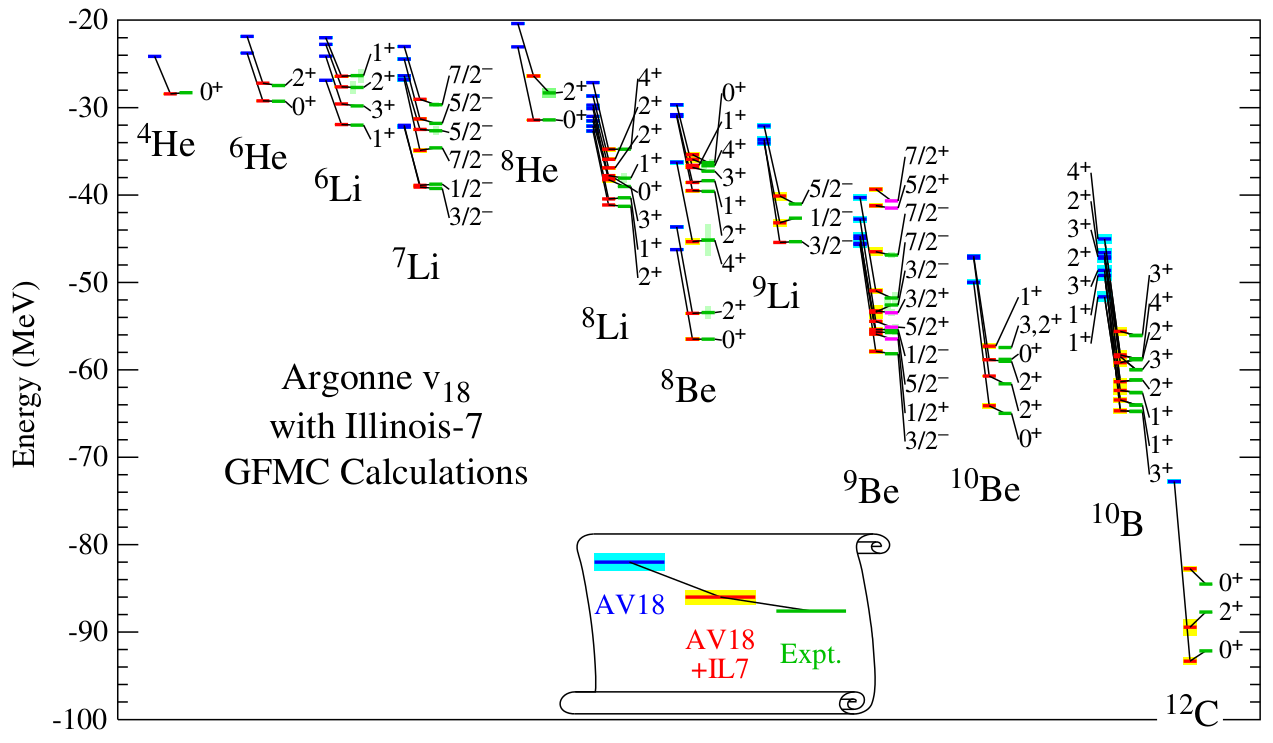
\includegraphics[width=\textwidth]{figures/gfmc_energies.png}
   \end{figure}
\end{frame}
\note{This was a recent review on QMC methods in nuclear physics from 2015. The IL7 is a 3N potential and the AV18 is the Argonne v18 potential. AV18 is a phenomenological potential. We use a subset of this potential. \red{Are these excited states?}}

\begin{frame}{Background}
\begin{itemize}
   \item We use the phenomenological potential AV6$'$, which is a subset of the AV18\footfullcite{wiringa1995} potential used in GFMC before.
   \begin{equation*}
      v_{ij} = \sum\limits_{p=1,6} v(r_{ij})\O{p}{ij}
   \end{equation*}
   \begin{equation*}
      \O{p=1,6}{ij} = 1, \ti\cdot\tj, \si\cdot\sj, (\si\cdot\sj)(\ti\cdot\tj), S_{ij}, S_{ij}(\ti\cdot\tj)
   \end{equation*}
   \begin{equation*}
      S_{ij} = 3(\si\cdot\mathbf{r_{ij}})(\sj\cdot\mathbf{r_{ij}})-\si\cdot\sj
   \end{equation*}
\end{itemize}
\end{frame}
\note{The $v_{18}$ potential also depends on spin and isospins. We use the Argonne $v_{6}$ potential which is a truncation of the Argonne $v_{18}$ potential.}

\section{Research}
\subsection{Quantum Monte Carlo}
\begin{frame}{Monte Carlo Integration}
\begin{itemize}
   \item We often want to solve multidimensional integrals.
      \begin{equation*}
         I=\int g(\R)d\R
      \end{equation*}
   \item We can rewrite this in terms of a probability distribution $P(\R)$.
      \begin{equation*}
         I=\int f(\R)P(\R)d\R
      \end{equation*}
   \item This looks like an expectation value of $f(\R)$. If the $\R_n$'s are pulled from $P(\R)$ then we can write this in discrete form as
   \begin{equation*}
      I=\lim\limits_{N\rightarrow\infty} \frac{1}{N}\sum\limits_{n=1}^N f(\R_n) \approx \frac{1}{N}\sum\limits_{n=1}^N f(\R_n)
   \end{equation*}
\end{itemize}
\end{frame}

\begin{frame}{Sampling $P(\R)$}
\begin{itemize}
   \item We need to draw samples from a probability density. If this is an function with an invertible CDF this is easy to do.
   \begin{columns}
      \begin{column}{0.7\textwidth}
      \begin{figure}[h]
         \centering
         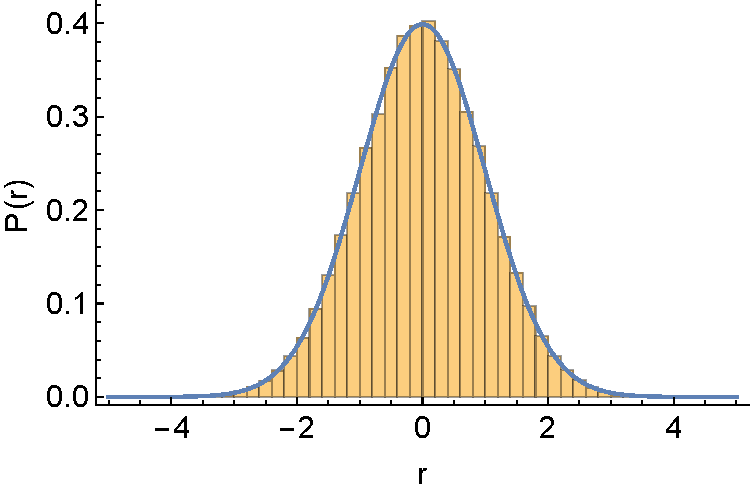
\includegraphics[width=\textwidth]{figures/gauss.pdf}
      \end{figure}
      \end{column}
      \begin{column}{0.4\textwidth}
      $r=\mathrm{CDF}^{-1}\left({\xi}\right)$
      \end{column}
   \end{columns}
   \item If not then we need to use other methods to sample the distribution.
\end{itemize}
\end{frame}

\begin{frame}{Metropolis Algorithm}
   The Metropolis algorithm is a Markov Chain method that does not depend on history except for the previous point.
\begin{enumerate}
   \item Start at a random position, $\R$.
   \item Propose a move to a new position $\R'$, pulled from a distribution $T(\R'|\R)$, where $T$ can be a Gaussian centered on the current position. %%%This makes sure that too large of steps aren't taken.
   \item The probability of accepting the move is given by
   \begin{equation*}
      A(\R'|\R) = \mathrm{min}\left(1,\frac{P(\R')T(\R|\R')}{P(\R)T(\R'|\R)}\right)
   \end{equation*}
   \item The move is accepted if $A\ge u$ where $u$ is a uniform random number between 0 and 1.
\end{enumerate}
\end{frame}
\note{Two conditions to have convergence to the correct distribution. 1: The steps must be able to get from any allowed state to any other in a finite amount of steps. 2: There cannot be cycles (ACBACBACB...), rejecting some steps gets rid of cycles.}

\begin{frame}{Variational Monte Carlo}
\begin{itemize}
   \item VMC starts with a trial wave function which includes variable parameters.
   \item The variational principle guarantees
   \begin{equation*}
      E_V = \frac{\int\psi_T^*(\R)H\psi_T(\R)d\R}{\int\psi_T^*(\R)\psi_T(\R)d\R} \le E_0
   \end{equation*}
   \item To use what we learned above we want this to look like this
   \begin{equation*}
      E_V = \int f(\R)P(\R) d\R \approx \frac{1}{N}\sum\limits_{n=1}^N f(\R_n)
   \end{equation*}
\end{itemize}
\end{frame}

\begin{frame}{Variational Monte Carlo}
   \begin{equation*}
      E_V = \int P(\R)E_L(\R) d\R
   \end{equation*}
\begin{itemize}
   \item We can do that if we multiply by $\Psi_T(\R)\Psi_T^{-1}(\R)$.
   \begin{align*}
      P(\R) &= \frac{|\Psi_T(\R)|^2}{\int|\Psi_T(\R)|^2d\R} \\
%      E_L(\R) &= \Psi_T^{-1}(\R) H \Psi_T(\R)
      E_L(\R) &= \frac{\Psi_T^*(\R) H \Psi_T(\R)}{\Psi_T^*(\R) \Psi_T(\R)}
   \end{align*}
   \item Now using Monte Carlo integration we can write
   \begin{equation*}
      E_V \approx \frac{1}{N} \sum\limits_{n=1}^N E_L(\mathbf{R_n}),
   \end{equation*}
   where the $\R_n$ are samples from $P(\R)$.
\end{itemize}
\end{frame}

\begin{frame}{Variational Monte Carlo}
\begin{itemize}
   \item The statistical error in the energy is then given in the typical way
   \begin{equation*}
      \sigma_{E_V} = \sqrt{\frac{\left<E_L^2\right>-\left<E_L\right>^2}{N}} \approx \sqrt{\frac{\left(\frac{1}{N}\sum\limits_{n=1}^NE_L^2(\R_n)\right) - \left(\frac{1}{N}\sum\limits_{n=1}^NE_L(\R_n)\right)^2}{N-1}}
   \end{equation*}
   \item We can then vary the parameters in the trial wave function and calculate this until we minimize the energy or statistical error, since $E_V \ge E_0$.
\end{itemize}
\end{frame}

\begin{frame}{Variational Monte Carlo - Implementation}
\begin{enumerate}
   \item Generate N configurations (walkers) distributed randomly.
   \item Loop over each walker and do the following
   \begin{enumerate}
      \setlength\itemsep{0.2em}
      \item Calculate $P(\R) = \left|\braket{\Psi_T}{\R}\right|^2$
      \item Propose a move $\R' = \R + \Delta\xi$, where $\xi$ could be a vector of random variable from a Gaussian.
      \item Calculate $P(\R') = \left|\braket{\Psi_T}{\R'}\right|^2$
      \item Calculate the probability of acceptance $A=\mathrm{min}\left(1,\frac{P(\R')}{P(\R)}\right)$
      \item If accepted then $\R \rightarrow \R'$, else the next position in the Markov Chain for that walker is the same as the last, namely $\R$
   \end{enumerate}
   \item Calculate observables and repeat steps 2 until energy is minimized or uncertainties are low enough.
\end{enumerate}
\end{frame}

\begin{frame}{Diffusion Monte Carlo}
\begin{itemize}
   \item Diffusion Monte Carlo uses a Green's function to diffuse walkers in imaginary time to estimate the ground state energy and wave function based on a trial wave function.
   \begin{equation*}
      H\Psi = i\hbar\frac{d\Psi}{dt} ~ \xrightarrow{\tau=it/\hbar} ~ H\Psi = -\frac{d\Psi}{d\tau}
   \end{equation*}
   Using separation of variables we can write
   \begin{equation*}
      \Psi(\R,\tau) = \sum\limits_{n=0}^{\infty} c_n\phi_n(\R) e^{-\tau(E_n-E_0)}
   \end{equation*}
   \item The long imaginary time limit of this goes to the ground state.
   \begin{equation*}
      \lim\limits_{\tau\rightarrow\infty} \Psi(\R,\tau) = c_0\phi_0(\R)
   \end{equation*}
\end{itemize}
\end{frame}
\note{We start DMC from the minimized $\psi_T$ and configurations from VMC.}

\begin{frame}{Diffusion Monte Carlo}
\begin{itemize}
   \item The propagated wave function can be written
   \begin{equation*}
      \braket{\R'}{\Psi_T(\tau)} = \int d\R \bra{\R'}e^{-(H-E_0)\tau}\ket{\R}\braket{\R}{\Psi_T(0)}
   \end{equation*}
   \item Now we use $e^{-H\tau}=e^{-V\tau/2}e^{-T\tau}e^{-V\tau/2}+\mathcal{O}(\tau^3)$ and break up the propogator into small time steps $\dt = \tau/N$.
   \begin{equation*}
      \braket{\R_N}{\Psi_T(\tau)} = \int d\R_1 \ldots d\R_N \left[\prod\limits_{i=1}^N G(\R_i,\R_{i-1},\Delta\tau)\right] \braket{\R_0}{\Psi_T(0)}
   \end{equation*}
   \begin{equation*}
      G(\R',\R,\Delta\tau) = \bra{\R'}e^{-(H-E_0)\Delta\tau}\ket{\R}
   \end{equation*}
\end{itemize}
\end{frame}

\begin{frame}{Diffusion Monte Carlo}
\begin{itemize}
   \item In the small $\dt$ limit this propogator can be split up with the kinetic term being used to diffuse the walkers along a random path.
   \begin{equation*}
      \bra{\R'}e^{-T\Delta \tau}\ket{\R} = \left(\frac{m}{2\pi\hbar^2\Delta\tau}\right)^{3A/2}e^{-m(\R'-\R)^2/2\hbar^2\Delta\tau}
   \end{equation*}
   \item The potential term can then be used as a weight in a branching algorithm.
   \begin{equation*}
      w(\R') = e^{-\left(V\left(\R'\right)+V\left(\R\right)-2E_0\right)\Delta\tau/2}%\bra{\R'}e^{-(V-E_0)\Delta\tau}\ket{\R}
   \end{equation*}
   \item Importance sampling improves the variance of the sampling and can be included with
   \begin{equation*}
      G(\R',\R,\Delta\tau) \rightarrow G(\R',\R,\Delta\tau)\frac{\braket{\R}{\Psi_I}}{\braket{\R'}{\Psi_I}}
   \end{equation*}
\end{itemize}
\end{frame}

\begin{frame}{Diffusion Monte Carlo}
Branching: Each walker can be deleted or multiply. The number of walkers that continues is equal to $\mathrm{int}\left(w(\R')+\xi\right)$, where $\xi$ is a uniform random number from $[0,1]$.
\begin{columns}
\begin{column}{0.4\textwidth}
\begin{figure}
   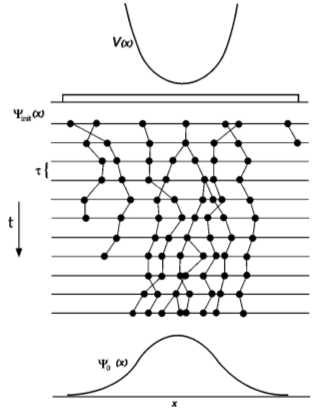
\includegraphics[width=0.9\textwidth]{figures/branch_full.png}
\end{figure}
\end{column}
\begin{column}{0.7\textwidth}
   {\color{blue}{Figure:}} Reprinted from W.M.C. Foulkes et al. \textit{Rev. Mod. Phys.,} 73:33-83, 2001.
\end{column}
\end{columns}
\end{frame}


\begin{frame}{Diffusion Monte Carlo - Implementation}
\begin{enumerate}
   \item Start with N configurations (walkers) from VMC
   \item Loop over each walker and do the following
   \begin{enumerate}
      \setlength\itemsep{0.2em}
      \item Propose a move, $\R' = \R + \chi$, where $\chi$ is a random number from the shifted Gaussian $\exp\left(\frac{m}{2\hbar^2\Delta\tau}\left(\R'-\R+2\frac{\nabla\Psi_I(\R')}{\Psi_I(\R')}\right)^2\right)$.
      \item The move is then accepted with the probability $A(\R'\leftarrow\R)=\mathrm{min}\left(1,\frac{\Psi_T^2(\R')}{\Psi_T^2(\R)}\right)$.
      \item Calculate the weight $w(\R')=\exp\left(-\left(E_L(\R')+E_L(\R)-2E_0\right)\Delta\tau/2\right)$.
      \item Do branching.
      \item Calculate and collect the observables and uncertainties needed and increase the imaginary time by $\Delta\tau$.
   \end{enumerate}
   \item Repeat from step 2 to 6 until the uncertainties are small enough.
\end{enumerate}
\end{frame}

\begin{frame}{Auxiliary Field Diffusion Monte Carlo - Spin Sampling}
\begin{itemize}
   \item AFDMC samples auxiliary fields to rotate the spins/isospins of the walkers.
   \item The spin/isospin dependent part of the potential is what is used in the spin/isospin dependent part of the propagator.
   \begin{equation*}
      G_{SD}(R'S',RS,\dt) = \bra {R'S'}e^{-V_{SD}\dt} \ket{RS}
   \end{equation*}
   \begin{equation*}
      V_{SD} = \sum\limits_{p=2}^6\sum\limits_{i<j}v_p(r_{ij})\Opij
   \end{equation*}
   \item For $v_6$, a truncation of the phenomenological Argonne $v_{18}$ potential, the operators are $\si\cdot\sj$, $\ti\cdot\tj$, $\si\cdot\sj \ti\cdot\tj$, $S_{ij}$ and $S_{ij} \ti\cdot\tj$, where $S_{ij} = 3\si\cdot\hat{r}_{ij}\sj\cdot\hat{r}_{ij}-\si\cdot\sj$
\end{itemize}
\end{frame}

\begin{frame}{Auxiliary Field Diffusion Monte Carlo - Spin Sampling}
\begin{itemize}
   \item The potential can be written in terms of matrices that are made of the $v_p(r_{ij})$, are symmetric, and 0 if $i=j$.
   \begin{equation*}
      V_{SD} = \frac{1}{2}\sum\limits_{i\alpha j\beta} \sigma_{i\alpha}A^{\sigma}_{i\alpha j\beta}\sigma_{j\beta}
      + \frac{1}{2}\sum\limits_{i\alpha j\beta} \sigma_{i\alpha}A^{\sigma\tau}_{i\alpha j\beta}\sigma_{j\beta}\ti\cdot\tj
      + \frac{1}{2}\sum\limits_{ij} A^{\tau}_{ij}\ti\cdot\tj
   \end{equation*}
   \item We can construct these matrices and then solve for their eigenvalues and eigenvectors.
\begin{align*}
   &\sum\limits_{j\beta} A^{\sigma}_{i\alpha j\beta}\psi^{\sigma}_{nj\beta} = \lambda^{\sigma}_n\psi^{\sigma}_{ni\alpha} \\
   &\sum\limits_{j\beta} A^{\sigma\tau}_{i\alpha j\beta}\psi^{\sigma\tau}_{n j\beta} = \lambda^{\sigma\tau}_n\psi^{\sigma\tau}_{ni\alpha} \\
   &\sum\limits_{j} A^{\tau}_{ij}\psi^{\tau}_{n,j} = \lambda^{\tau}_n\psi^{\tau}_{ni}
\end{align*}
\end{itemize}
\end{frame}

\begin{frame}{Auxiliary Field Diffusion Monte Carlo - Spin Sampling}
\begin{itemize}
   \item The potential can then be written in terms of the square of new single particle operators.
   \begin{equation*}
      V_{SD} = \frac{1}{2}\sum\limits_{n=1}^{3A} \left(O_{n}^{\sigma}\right)^2 \lambda_n^{\sigma}
      + \frac{1}{2}\sum\limits_{\alpha=1}^{3}\sum\limits_{n=1}^{3A} \left(O_{n\alpha}^{\sigma\tau}\right)^2 \lambda_n^{\sigma\tau}
       + \frac{1}{2}\sum\limits_{\alpha=1}^{3}\sum\limits_{n=1}^{A} \left(O_{n\alpha}^{\tau}\right)^2 \lambda_n^{\tau}
   \end{equation*}
   \begin{equation*}
   \begin{split}
      O_{n}^{\sigma} &= \sum\limits_{j\beta} \sigma_{j\beta}\psi_{nj\beta}^{\sigma} \\
      O_{n\alpha}^{\sigma\tau} &= \sum\limits_{j\beta} \tau_{j\alpha}\sigma_{j\beta}\psi_{nj\beta}^{\sigma\tau} \\
      O_{n\alpha}^{\tau} &= \sum\limits_{j} \tau_{j\alpha}\psi_{nj}^{\tau}
   \end{split}
   \end{equation*}
\end{itemize}
\end{frame}

\begin{frame}{Auxiliary Field Diffusion Monte Carlo - Spin Sampling}
\begin{itemize}
   \item Since we have squared single particle operators in the propagator we can now rewrite the propagator in terms of the Hubbard-Stratanovich transformation.
   \begin{equation*}
      e^{-\frac{1}{2}\lambda O^2} = \frac{1}{\sqrt{2\pi}} \int dx e^{-\frac{x^2}{2} + \sqrt{-\lambda}xO}
   \end{equation*}
   \item Since we have 15A operators ($3A$ for $O_{n}^{\sigma}$, $9A$ for $O_{n\alpha}^{\sigma\tau}$, and $3A$ for $O_{n\alpha}^{\tau}$), the spin-isospin dependant part of the propagator becomes
   \begin{equation*}
      G_{SD}(R'S',RS,\dt) = \prod\limits_{n=1}^{15A}\frac{1}{\sqrt{2\pi}}\int dx_n e^{-\frac{x_n^2}{2}}e^{\sqrt{-\lambda_n\dt} x_nO_n}.
   \end{equation*}
\end{itemize}
\end{frame}

\subsection{Trial Wave Function}
\begin{frame}{Slater Determinant}
\begin{itemize}
   \item The simplest wave function for a many-fermion system is a Slater determinant.
   \begin{equation*}
      \psi_{T} = \mathcal{A} \prod\limits_{i=1}^A \phi_i(\mathbf{r}_i,s_i) = \frac{1}{A!} \mathrm{det}~\phi_i(\mathbf{r}_i,s_i)
   \end{equation*}
   \item Short range correlations need to be put in by hand via Jastrow-like correlations.
   \begin{equation*}
      \ket{\psi_T} = \prod\limits_{i<j}f(r_{ij}) \ket{\phi},
   \end{equation*}
   where $\braket{RS}{\phi}$ is the Slater determinant described above.
\end{itemize}
\end{frame}

\begin{frame}{Full Trial Wave Function}
\begin{itemize}
   \item A completely cluster decomposable ($\ket{\Phi_A+\Phi_B} = \ket{\Phi_A}\ket{\Phi_B}$) set of spin-isospin dependent correlations could be an exponential
   \begin{equation*}
       \ket{\psi_T} = \prod\limits_{i<j}f_c(r_{ij}) e^{\sum\limits_p\fpij\Opij} \ket{\phi}.
   \end{equation*}
   \item However, a symmetrized product wave function captures almost the same physics.
   \begin{equation*}
      \ket{\psi_T} = \left[\prod\limits_{i<j}f_c(r_{ij})\right]\left[\mathcal{S}\prod\limits_{i<j}\left(1+\sum\limits_p \fpij\Opij\right)\right]\ket{\phi}
   \end{equation*}
\end{itemize}
\end{frame}

\begin{frame}{Quadratic Correlations}
\begin{itemize}
   \item If we assume the correlations are small we can expand this exponential to first order.
   \begin{equation*}
      \ket{\psi_T} = \prod\limits_{i<j}f_c(r_{ij}) \left(1+\sum\limits_p\fpij\Opij\right) \ket{\phi}
   \end{equation*}
   \item By expanding the product you can write this as
   \begin{equation*}
   \begin{split}
      \ket{\psi_T} &= \left[\prod\limits_{i<j}f_c(r_{ij})\right] \left[1+\fOpij\right. \\
      & + \left.\frac{1}{2}\fOpij\fOqklquad + \ldots \right] \ket{\phi}
   \end{split}
   \end{equation*}
\end{itemize}
\end{frame}

\begin{frame}{Independent Pair Correlations}
\begin{itemize}
   \item Or it can be expanded to get independent pair terms
   \begin{equation*}
   \begin{split}
      \ket{\psi_T} &= \left[\prod\limits_{i<j}f_c(r_{ij})\right] \left[1+\fOpij\right. \\
      & + \left.\beta\fOpij\fOqklip + \ldots \right] \ket{\phi}
   \end{split}
   \end{equation*}
\end{itemize}
\begin{figure}[h]
   \centering
   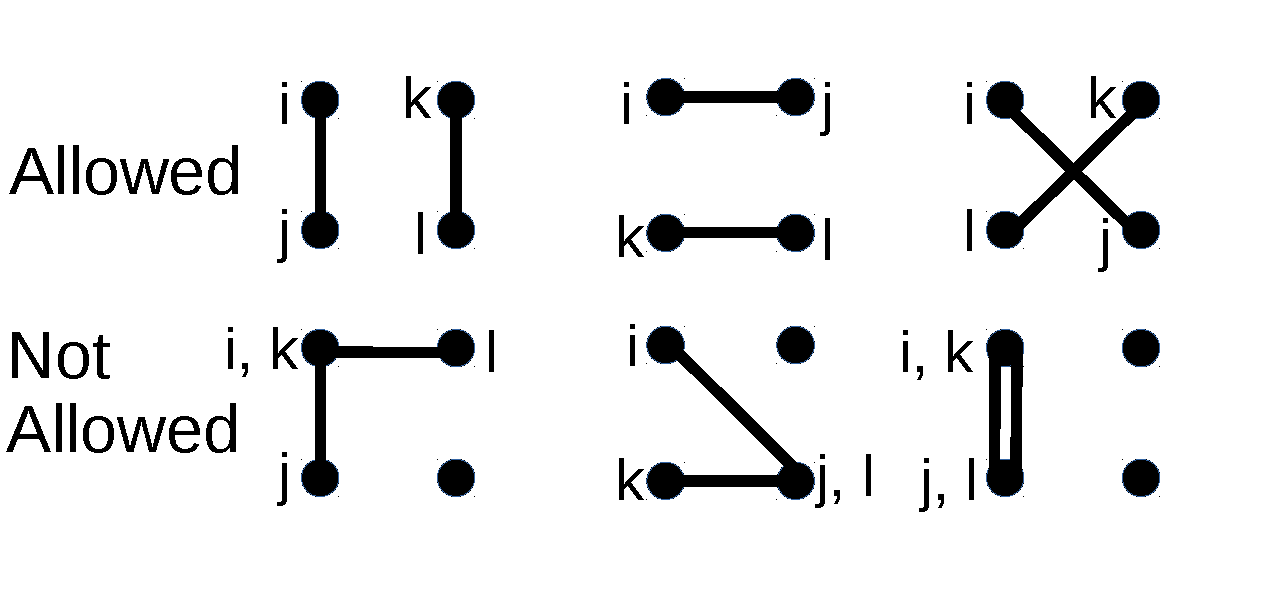
\includegraphics[width=0.7\textwidth]{figures/pairing.pdf}
\end{figure}

\end{frame}

\subsection{Results}
\begin{frame}{Results}
\begin{figure}[h]
   \centering
   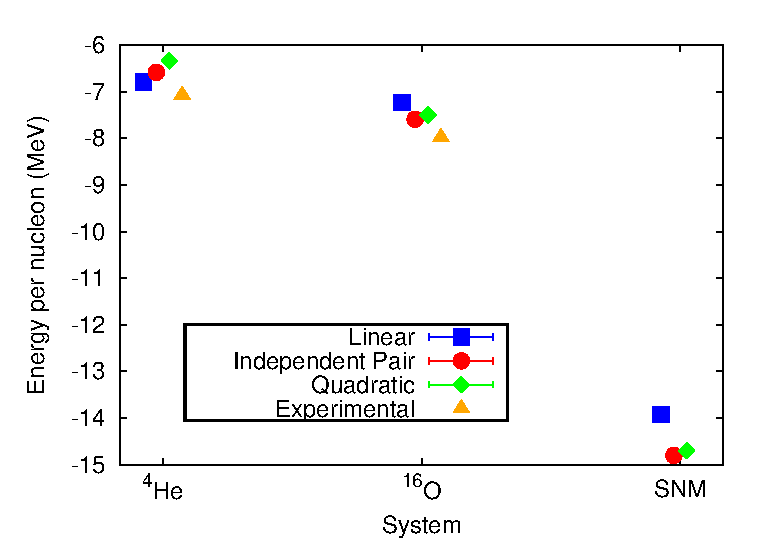
\includegraphics[width=0.5\textwidth]{figures/energy.eps}
\end{figure}
\begin{table}[h!]
   \centering
   \scalebox{0.8}{
   \begin{tabular}{ccccc}
      \hline \hline
      & Linear & IndPair & Quadratic & Expt.\\
      \hline
      $^4$He & -27.17(4) & -26.33(3) & -25.35(3) & -28.295\\
      $^{16}$O & -115.7(9) & -121.5(1.5) & -120.0(1.4) & -127.619\\
      SNM($\rho=0.16$ fm$^{-1}$) & -13.92(6) & -14.80(7) & -14.70(11) & \\
      \hline \hline
   \end{tabular}
   }
   \\ Energies (per nucleon) in MeV, SNM was done with 28 particles with periodic boundary conditions.
\end{table}
\end{frame}

\begin{frame}{Results}
\begin{figure}[h]
   \centering
   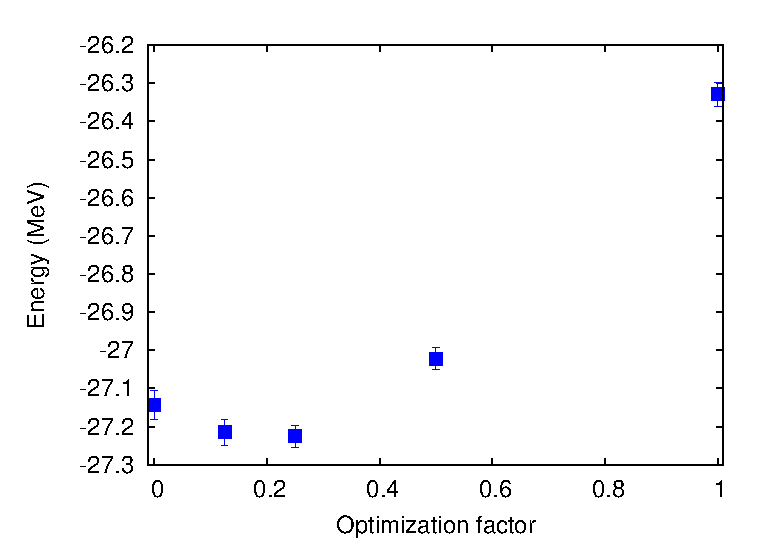
\includegraphics[width=0.7\textwidth]{figures/quadfact.eps}
\end{figure}
Optimization of quadratic $\beta$ parameter for $^{4}$He with independent pair correlations.
\end{frame}

\begin{frame}{Results}
\begin{columns}
\begin{column}{0.55\textwidth}
\begin{figure}[h]
   \centering
   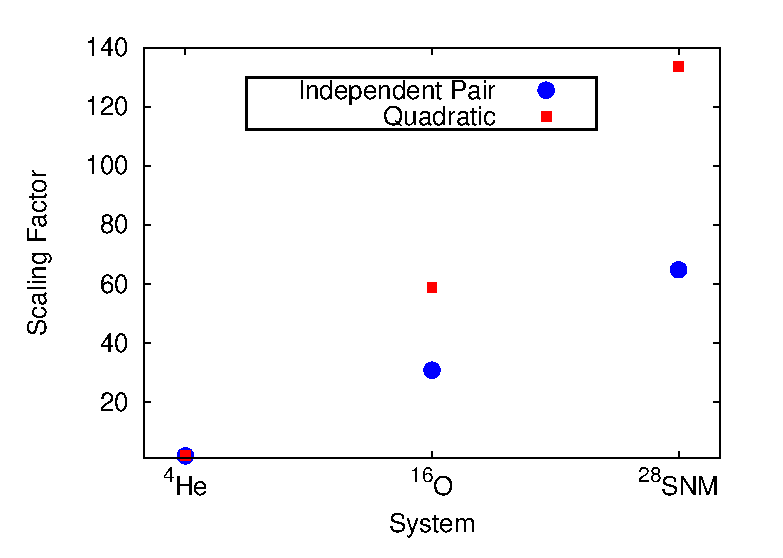
\includegraphics[width=\textwidth]{figures/scaling.eps}
\end{figure}
\end{column}
\begin{column}{0.55\textwidth}
\begin{figure}[h]
   \centering
   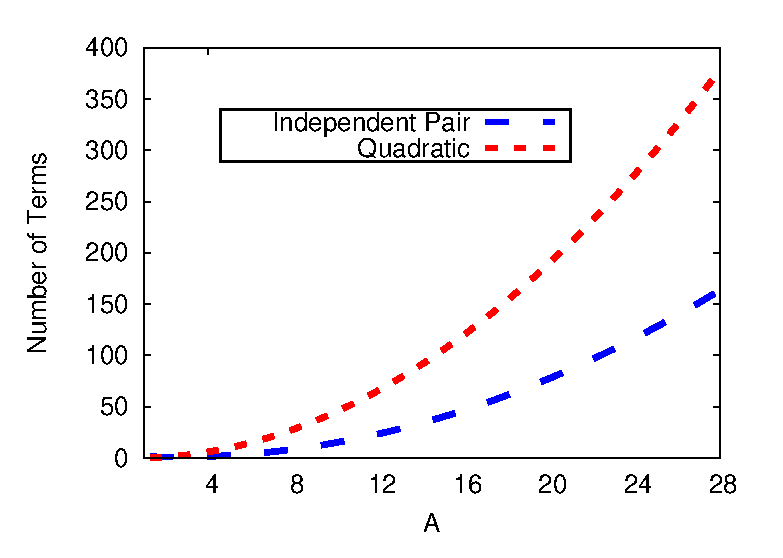
\includegraphics[width=\textwidth]{figures/scaling_theory.eps}
\end{figure}
\end{column}
\end{columns}
\begin{table}[h!]
   \centering
   \begin{tabular}{cccc}
      \hline \hline
       & $^{4}$He & $^{16}$O & SNM(28)\\
      \hline
      Independent Pair & 1.73 & 30.7 & 64.8 \\
      Quadratic & 2.00 & 58.8 & 133.6 \\
      \hline \hline
   \end{tabular}
\end{table}
\end{frame}

\section{Conclusion}
\subsection{Conclusion}
\begin{frame}{Conclusion}
\begin{itemize}
   \item We have added independent pair and full quadratic correlations to the already linearly correlated wave function.
   \item The addition of these operators decreases the energy for each system.
   \item Though there was not a large difference between independent pair and full quadratic correlations the scaling was about twice as good for independent pair correlations.
\end{itemize}
\end{frame}

\begin{frame}{End of Comprehensive}
   Questions?
\end{frame}

\section{Prospectus}
\begin{frame}{Outlook}
\begin{itemize}
   \item{I will apply these calculations to other medium mass nuclei.}
   \begin{itemize}
      \item $^{40}$Ca
      \item Other isotopes of Oxygen
      \item Open shell nuclei
   \end{itemize}
   \item This work will then be published.
   \begin{itemize}
      \item Draft by the end of the summer.
   \end{itemize}
   \item When this project is done I plan to move on to one or more additional projects.
\end{itemize}
\end{frame}

\subsection{Exponential Correlations}
\begin{frame}{Exponential Correlations}
\begin{itemize}
   \item Another way to improve the trial wave function is to start with the exponential correlations and use the Hubbard-Stratanovich transformation to sample them, just like we do for the spin-isospin part of the propagator in AFDMC.
   \begin{align*}
       \ket{\psi_T} &= \prod\limits_{i<j}f_c(r_{ij}) e^{\sum\limits_p\fpij\Opij} \ket{\phi} \\
%       \ket{\psi_T} &= \left[\prod\limits_{i<j}f_c(r_{ij})\right] e^{\sum\limits_p\sum\limits_{i<j}\fpij\Opij} \ket{\phi}
   \end{align*}
\end{itemize}
\end{frame}

\begin{frame}{Exponential Correlations}
\begin{itemize}
   \item Compare what we have for the potential (without the Jastrow part) to what we have for the Green's function.
   \begin{align*}
       \braket{\psi_T}{RS} &= \bra{\phi} e^{\sum\limits_p\sum\limits_{i<j}\fpij\Opij} \ket{RS} \\
      G_{SD}(R'S',RS,\dt) &= \bra {R'S'} e^{\sum\limits_p\sum\limits_{i<j}u_p(r_{ij})\Opij\dt} \ket{RS}
   \end{align*}
   \item The only differences between these are the different function $u$ and $f$, and the $\dt$. Then the correlations in the trial wave function can be written as
   \begin{equation*}
      e^{\sum\limits_p\sum\limits_{i<j}\fpij\Opij} = \prod\limits_{n=1}^{15A}\frac{1}{\sqrt{2\pi}}\int dx_n e^{-\frac{x_n^2}{2}}e^{\sqrt{-\lambda_n} x_nO_n}.
   \end{equation*}
\end{itemize}
\end{frame}

\begin{frame}{Exponential Correlations}
\begin{itemize}
   \item To improve the variance of sampling the average of with samples $x$ and $-x$ is taken.
   \item This improved wave function will allow us to study larger nuclear system like neutron-rich nuclei created by the r-process.
\end{itemize}
\end{frame}

\subsection{Clustering in Nuclear Matter}
\begin{frame}{Particle Clustering in Nuclear Matter}
\begin{itemize}
   \item When a nucleus has an even number of $n$ and $p$ each $n$ pairs with a $p$, and this decreases the energy of the system.
   \item However two $n$ and two $p$ can pair together to form an $\alpha$-particle.
   \item At low densities quartetting is more energetically favorable than pairing\footfullcite{schuck2013_1}.
   \item I want to show that we can see this clustering.
   \item I also want to do calculations at different densities to study how these clusters dissolve as a function of density.
\end{itemize}
\end{frame}
\note{For example we see this in the Liquid-drop model}

\begin{frame}{Neutron Star}
\begin{columns}
\begin{column}{0.55\textwidth}
\begin{figure}
   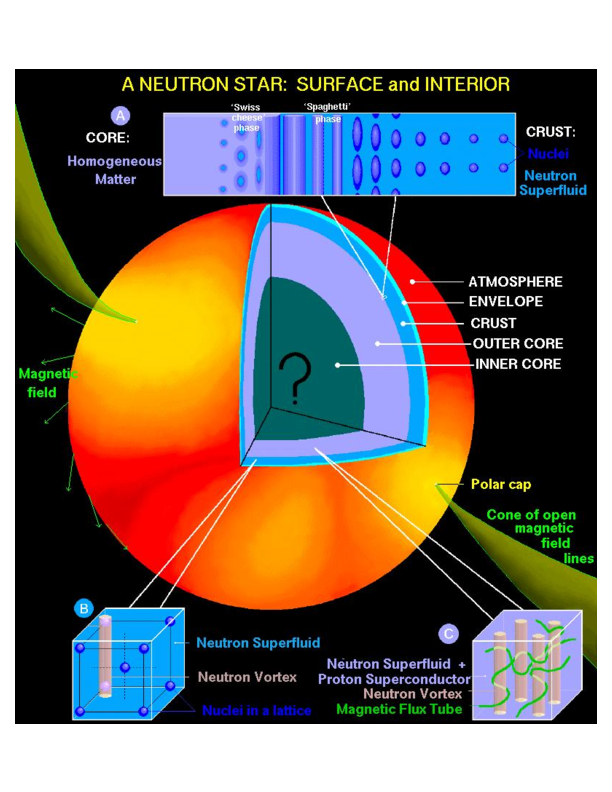
\includegraphics[width=0.9\textwidth]{figures/neutronstar.png}
\end{figure}
\end{column}
\begin{column}{0.4\textwidth}
   {\color{blue}{Figure:}} Reprinted from Dany Page et al. \textit{Annu. Rev. Nucl. Part. Sci.,} 56:327-374, 2006.
\end{column}
\end{columns}
\end{frame}

\begin{frame}{Particle Clustering in Nuclear Matter}
\begin{itemize}
   \item Calculate the energy/particle ($E_{14n}/14$) of pure neutron matter with 14 particles in a periodic box and compare with 14 neutrons plus 2 protons ($E_{14n2p}/16$).
   \item If there is quartetting there should be a shift in the energy.
   \begin{equation*}
      E_{14n2p}/16 \approx (E_{12n}+E_{\alpha})/16
   \end{equation*}
   \item If neutron matter had energy $E_n/N \approx 15$MeV and the alpha $E_\alpha \approx -28$MeV this would be
   \begin{equation*}
      E_{14n2p}/16 \approx \left(15\frac{\mathrm{MeV}}{part}\cdot12-28\mathrm{MeV}\right)/16 = 4 \mathrm{MeV}
   \end{equation*}
\end{itemize}
\end{frame}

\begin{frame}{Particle Clustering in Nuclear Matter}
   \red{Here put something about the g(r) pair distrubitions}
\end{frame}

\subsection{Outlook}
\begin{frame}{Timetable}
\begin{tabular}{p{2cm}|p{8cm}}
\\[-1.5ex]Summer 17 & ~Submit draft for quadratic correlations paper \\[1.5ex]
\hline \\[-1.5ex]
Fall 17 & ``Complete" exponential correlations project \\[1.5ex]
\hline \\[-1.5ex]
Spring 18 & ``Complete" alpha clustering project \\[1.5ex]
\hline \\[-1.5ex]
Summer 18 & ~Submit a draft of alpha clustering paper \\[1.5ex]
\hline \\[-1.5ex]
Fall 18 & ~Start writting dissertation \\[1.5ex]
\hline \\[-1.5ex]
Spring 19 & ~Finish dissertation and defence \\[1.5ex]
\end{tabular}
\end{frame}

\begin{frame}{Available Resourses}
\begin{itemize}
   \item Current Allocation: 250,000 hours on LSU SuperMIC (XSEDE)
   \begin{itemize}
      \item Quadratic Correlations: 
   \end{itemize}
   \item Proposed Allocation: 500,000 hours on LSU SuperMIC (XSEDE)
   \begin{itemize}
      \item Exponential Correlations: 
      \item Alpha Clustering: 
   \end{itemize}
\end{itemize}
\end{frame}

\begin{frame}{Dissertation Breakdown}
\begin{enumerate}
   \item Introduction
%   \begin{enumerate}
%      \item Background/Motivation
%      \item Outline
%   \end{enumerate}
   \item Methods
   \begin{enumerate}
      \item Variational Monte Carlo
      \item Diffusion Monte Carlo
      \item Auxiliary Field Diffusion Monte Carlo
      \item Hamiltonian
   \end{enumerate}
   \item Trial Wave Function
   \begin{enumerate}
      \item Expand the Symmetric Product Wave Function
      \item Exponential Wave Function
      \item Comparing Trial Wave Functions
   \end{enumerate}
   \item Alpha Clustering in Nuclear Matter
   \begin{enumerate}
      \item Theory
      \item Results
   \end{enumerate}
   \item Conclusion
%   \begin{enumerate}
%      \item Summary
%      \item Outlook
%   \end{enumerate}
\end{enumerate}
\end{frame}

\end{document}
